\chapter{Essence Reflection Meetings}
\section{Abstract}

This paper presents an empirical evaluation of the team reflection support provided by the Software Engineering Method and Theory (SEMAT) Essence framework, and compares Essence reflection meetings to other types of team reflection meetings. The researchers conducted a field study involving seven graduate master student teams running Essence reflection meetings throughout their practicum projects aiming at delivering a working product for an industry client. The main result validates that Essence meetings generate reflective team discussions through a thinking framework that is holistic, state-based, goal- driven, and method-agnostic. Student teams benefit from stepping back and assessing the project holistically throughout its lifecycle. The goals set by the framework's checklists lead the teams to address critical aspects of the project that have not been considered. All team members are encouraged to express their views and influence the various project dimensions. Essence reflection meetings are comparable and complementary to Agile retrospectives, and project teams might want to leverage both techniques. The value added by Essence reflections is to surface unknown issues, help monitor progress, steer the project to a higher state, and prevent retrospectives from being repetitive by varying styles.

\section{Introduction}

The authors investigated a novel approach to monitoring and steering software development projects provided by the Software Engineering Method and Theory (SEMAT) Essence framework \cite{SEMATKernel}. Among the various benefits, team reflection stands out as being the most appreciated aspect of the approach from a student point of view. Therefore this paper elaborates on this result by focusing specifically on Essence team reflection.

There exists different types of reflection meetings. Some, like post-mortems or project retrospectives, are conducted once at the end of the project (or release). Others, like Agile retrospectives, are conducted throughout the project lifecycle, typically at the end of each iteration or Sprint. There are many variations or styles of Agile retrospectives \cite{Derby2006, KuaRetrospectiveHandbook}, and different authors refer to them using different names, including iteration retrospectives, Sprint retrospectives, or heartbeat retrospectives. In this paper we explain why Essence reflection meetings are comparable to Agile retrospectives, highlight the similarities and differences between the two, and suggest how project teams could leverage both techniques in a complementary fashion.

This paper introduces the SEMAT's Essence framework, presents the field study, and reports on the field study results with a focus on team reflection.

\section{SEMAT Essence Overview}
The core idea of the Software Engineering Method and Theory (SEMAT) Essence framework \cite{SEMATKernel} is that software projects exhibit universal behavior and transition through identifiable states as they progress. The states are grouped by software engineering dimensions called \quotes{alphas.} Essence identifies seven alphas as core to every software engineering project: \textbf{Stakeholders}, \textbf{Opportunity}, \textbf{Requirements}, \textbf{Software System}, \textbf{Team}, \textbf{Way of Working}, and \textbf{Work}. These seven alphas serve as the Essence kernel. Each alpha progresses through a number of states during the project lifecycle. For example, the \textbf{Stakeholders} alpha progresses through the states \textit{Recognized}, \textit{Represented}, \textit{Involved}, \textit{In Agreement}, \textit{Satisfied for Deployment}, and \textit{Satisfied in Use}. Each state includes a checklist to help determine if the project has achieved that state or not. Table \ref{EssenceReflectionMeetings} shows the checklist related to the Bounded state of the \textbf{Requirements} alpha.




\section{Field Study Description}
The field study aims at evaluating the effectiveness of the SEMAT Essence's approach. A complete description is available in \cite{ICSE2014}. The study includes seven student teams: three geographically distributed student teams and four co-located student teams. Each team worked on creating or evolving a software solution for a different industry client, like an electric car fleet management system or a survivable social network. By design, the projects had a medium to high level of technical complexity, as they often involved multiple technologies or platforms or integrate with legacy systems. The practicum projects ran for 12 to 15 weeks, during which each student dedicated about 20 hours per week to the project. Students worked in teams of two to five members. Teams determined their own software development approach. Most students had a reasonable knowledge of a diverse set of generally accepted software engineering practices, and the ability to execute these practices somehow effectively. All projects adopted an iterative lifecycle.
   
The teams were asked to leverage Essence throughout their project. Each team met on a regular basis (mostly weekly) for a 30 minutes Essence session. During each session, the team covered most or all of the alphas. For each alpha, the team identified their project current state, target state, and any work items necessary to transition from the current to the target state. In order to avoid anchoring bias, the current state identification was performed using a \quotes{poker game} approach \cite{ICSE2014}. In that context, each participant secretly determines the current state and all reveal their current state at the same time. In case of disagreement, the team discusses the different points of view until the participants reach an agreement. Table \ref{EssenceReflectionMeetings} provides a conceptual representation of how Essence was used in practice by each team.

A faculty member was present to facilitate each session. Faculty involvement was kept to a minimum to limit influencing the students. The faculty's role was constrained to recording progress, guiding the team through the application of the approach, and validating the objectivity of the team's self-assessment of their project state. At the end of each project a survey was sent to the students to collect their feedback on the application of the approach.

The qualitative and quantitative value of Essence refection meetings was measured primarily based on students' feedback collected during the weekly meetings and final survey.

\section{Field Study Results}
\textbf{Research Question:} How does Essence support team reflection?

The original intent of each Essence session was to monitor the team's progress and steer the project towards higher Essence states. The sessions also provided a natural setting for team reflection. Indeed, a majority of students (72\%) spontaneously mentioned reflection or retrospectives in the survey responses (80\% of the students participated in the survey).

For instance, one student mentioned: \participantQuote{What I liked most about Essence is that it invoked reflective discussion.} Another student mentioned: \participantQuote{The team was pleased to see that Essence also covered `The Way of Working' as well as `The Team'. These two topics generated useful team introspection at the beginning of the practicum and were nice reminders that the team does constant checkups for the overall condition of the members and the project.} Overall, the survey responses touch upon the following key ingredients of Essence reflection meetings:

\textbf{Holistic Thinking Framework}. The seven alphas, together with their states and checklists, provide the team with a thinking framework encouraging the team to think about the project in a holistic fashion, based on seven project dimensions (a.k.a. alphas). One student noted: \participantQuote{Essence enabled the team to keep an eye on the status of the project by zooming out and assessing the overall picture.} Stepping back and looking at the project holistically provides the distance and perspectives needed to understand a situation, reflect, and make informed decisions.

\textbf{State-based \& Goal-driven Thinking Framework}. The Essence thinking framework evolves throughout the project lifecycle, based on the project's specific alpha states. At each state, new checklist items (goals) are presented to the team, encouraging the team members to think about and address aspects of the project that are relevant to the current state. One student noted: \participantQuote{I like the fact that Essence provides a structured way of thinking about critical aspects of the project at different stages of the project.}

\textbf{Team Discussion}. Essence reflection meetings enable all team members to express their views and influence the different aspects of the project. Here is an illustrating quote: \participantQuote{Essence meetings allowed everyone on the team to have a say in the different aspects of the project.} Another student added: \participantQuote{It allows us to reflect on where we stand in the project and remind us of the points we are missing.}

\begin{figure}[t]
\centering
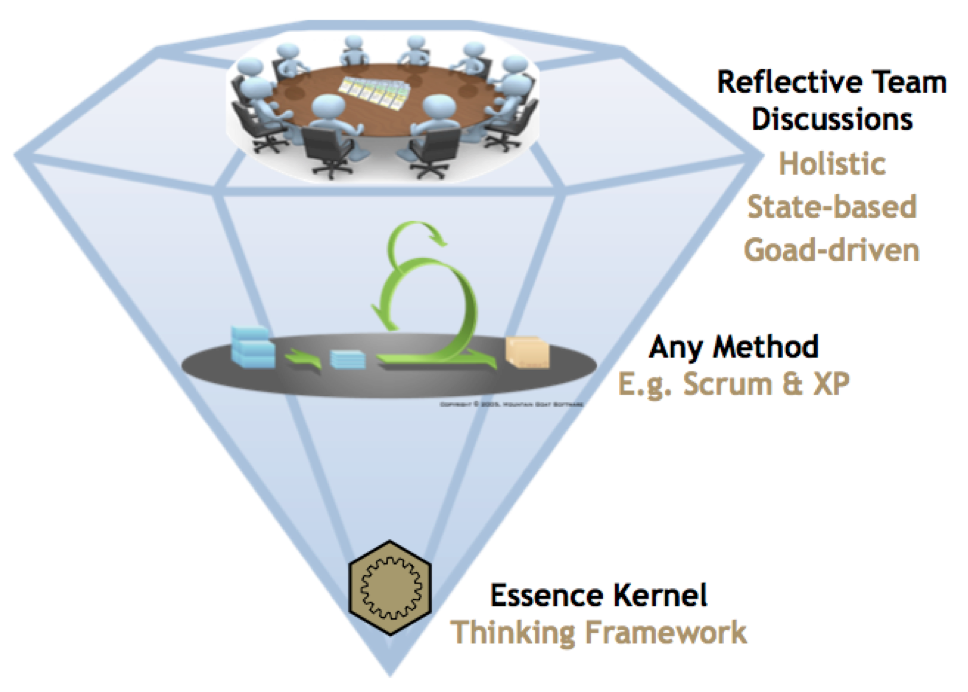
\includegraphics[width=3.4in]{reflection_meeting_images/EssenceDiamondEffect.png}
\caption{ Essence kernel's diamond effect}
\label{EssenceDiamondEffect}
\end{figure}

\textbf{Method-Agnostic}. The team decides what to do to reach the goals set by the target states. The team has the flexibility to leverage any software development method or set of practices that best suit their needs. This is illustrated in Figure \ref{EssenceDiamondEffect} with the Essence kernel's \quotes{diamond effect,} where the kernel alphas \quotes{radiate} to enable reflective discussions touching the many facets of the project throughout its lifecycle, independently of the software development method adopted by the team.

In conclusion, Essence supports team reflection by generating reflective team discussions through a thinking framework that is holistic, state-based, goal-driven, and method-agnostic. The teams benefit from stepping back and assessing the project holistically throughout its lifecycle. The goals set by the alpha state checklists lead the team to address critical aspects of the project that have been neglected. These aspects go beyond technology by including elements like \textbf{Team}, \textbf{Way of Working}, or \textbf{Stakeholders}.

\textbf{Research Question}: How does Essence reflection meetings compare to other types of reflection meetings?

Essence reflection meetings follow a state-based approach, with states covering the entire project lifecycle. Consequently, Essence reflection meetings are most effective if conducted on a regular basis throughout the entire project lifecycle. Therefore, Essence reflection meetings are not comparable to post-mortems or project retrospectives that are conducted only once at the end of the project (or release). Essence reflection meetings could be compared to Agile retrospectives \cite{Derby2006, KuaRetrospectiveHandbook}, because they are also conducted throughout the project lifecycle, typically at the end of each iteration or Sprint.

In this section we are comparing Agile retrospectives and Essence reflection meetings in terms of purpose, frequency, duration, structure, content, outcome, and facilitation concerns.

\textbf{Purpose}. The goal of an Agile retrospective is for the team to contemplate what worked and did not work during the last iteration in order to adapt the methods and teamwork moving forward. The focus is mostly on the past. The goal of an Essence reflection is for the team to consider various project dimensions in order to bring the whole project towards a higher state. The focus is mostly on the future.
  
\textbf{Frequency}. Both Agile retrospectives and Essence reflections can be conducted at the end of an iteration or Sprint, or at other intervals defined by the project team. During our field study, each team generally met on a weekly basis. We recommend frequent sessions early in the project when many issues arise. Later on, once a team becomes a high-performing team producing high quality outcome, the team needs less support and the frequency of the sessions could decrease.

\textbf{Duration}. Both Agile retrospectives and Essence reflections can be time boxed to a short session ranging from 30 minutes to a few hours. During our field study, each team generally met for a 30- minute session. We recommend adjusting the duration based on the team size and any other known parameters that might influence the length of the conversations, like team dynamic, issues and uncertainty, or session frequency.

\textbf{Structure}. While facilitators may run Agile retrospectives differently, many adopt a structure similar to the one proposed by Derby and Larsen in \cite{Derby2006}. Derby and Larsen generalize the stages of Agile retrospectives as: (1) Set the stage, (2) Gather data, (3) Generate insights, (4) Decide what to do, and (5) Close the retrospective. Even though Agile retrospectives and Essence reflections have a different structure, there are some similarities. During an Essence reflection meeting, the team repeats the key steps of gathering of data, generation of insights, and deciding what to do for each alpha. With the Essence kernel's seven alphas, this produces seven focused passes through the Agile retrospective stages. This structure is illustrated in Table \ref{ReflectionMeetingStructure}.

\begin{table}[t]
\renewcommand{\arraystretch}{1.5}
\centering
\caption{Essence reflection meeting structure}
\label{ReflectionMeetingStructure}
\begin{tabular}{p{3in}}
\hline
\textbf{Set the stage} (done informally) \\
\textit{For each alpha}:
  \begin{itemize}
  \item \textbf{Gather data (alpha states)} 
  
   Discuss alpha-related work since last session
   and agree on current and target states
  
  \item \textbf{Generate insights}

  Understand \textit{why} the target state is not achieved
  
  \item \textbf{Decide what to do}
  
  Set some goals to reach the target state 
  and agree on how to reach the goals

  \end{itemize}
    
\textbf{Close the retrospective} (done informally) \\
\hline
\end{tabular}
\end{table}


\textbf{Content}. One difference between Agile retrospectives and Essence reflections relates to the elicitation of topics to be covered during a session. During Agile retrospectives the topics discussed are elicited by the participants, while during Essence reflections the topics are determined by the alphas and their corresponding checklists. Issues emerge once the related alphas are covered. As a consequence, Agile retrospectives tend to focus on known issues while Essence reflections tend to make unknown issues apparent by covering the project holistically and reminding participants of \participantQuote{critical areas that are sometimes neglected.}

\textbf{Outcome}. Both Agile retrospectives and Essence reflections result in a small number of work items to be addressed, ideally before the next session. During an Agile retrospective, participants typically generate many possible work items that are prioritized and then limited to a few high value items to be addressed during the next iteration. During our field study, an average of 5 work items were generated per session. The identified work items were added to the team's work item list or backlog, and fed into the next planning activity when applicable.

\textbf{Facilitation}. Both Agile retrospectives and Essence reflections benefit from being conducted by an experienced and neutral facilitator. While this is often recommended for Agile retrospectives \cite{KuaRetrospectiveHandbook}, the need for a facilitator is reduced with Essence reflections as the Essence alphas and their checklists guide the discussions. A facilitator is only required during the initial sessions for training purposes. Similarly, it is generally recommended to prepare for Agile retrospectives ahead of time \cite{Derby2006, KuaRetrospectiveHandbook}. Essence reflection meetings might require the facilitator to print the cards ahead of time. We are currently leveraging an open source tool (available at http://essence.sv.cmu.edu) developed internally that provides digital cards, hence freeing us from any preparation. With such a tool, Essence reflection meetings are conducted very effectively with geographically distributed teams.

In conclusion, Essence reflection meetings could be compared to Agile retrospectives. Despite similarities between the two approaches, there are some key differences in terms of purpose and content. While Agile retrospectives aim at inspecting the last iteration in order to adapt the methods and teamwork (with a focus on the past), Essence reflections aim at considering various project dimensions in order to bring the whole project towards a higher state (with a focus on the future). While most styles of Agile retrospectives tend to focus on known issues, Essence reflections tend to make unknown issues apparent by covering the project holistically and reminding participants of critical areas that might be overlooked. These differences make Essence reflections and Agile retrospectives complementary. This is illustrated by the following student quote: \participantQuote{Though the team was holding retrospectives every week already, having Essence discussions be a part of it allowed the team to touch on important aspects of the project; aspects which would otherwise be ignored.}

\section {Conclusion}
Essence reflections are valuable and complementary to Agile retrospectives. Facilitators and project teams might want to leverage both. For instance, one might decide to conduct regular Essence reflection meetings during project initiation when the monitoring and steering mechanisms are the most effective \cite{ICSE2014}, then alternate between Essence reflections and other styles of Agile retrospectives. The value added by Essence reflections is to surface unknown issues, help monitor and steer the project towards a higher state, and prevent retrospectives from being repetitive by varying styles.

The results presented in this paper are limited to Essence reflection meetings with a facilitator. More research is necessary to assess the meetings' effectiveness without facilitators. Following the field study, we have been observing eight additional practicum teams. Our observations are consistent with the ones presented in the paper. We continue to collect data to evaluate the SEMAT Essence's framework with a focus on both effectiveness of the approach and accuracy of the model.

\begin{table*}[t]
\caption{How Essence is used in practice by a student team}
\centering
\begin{tabular}{l|l}
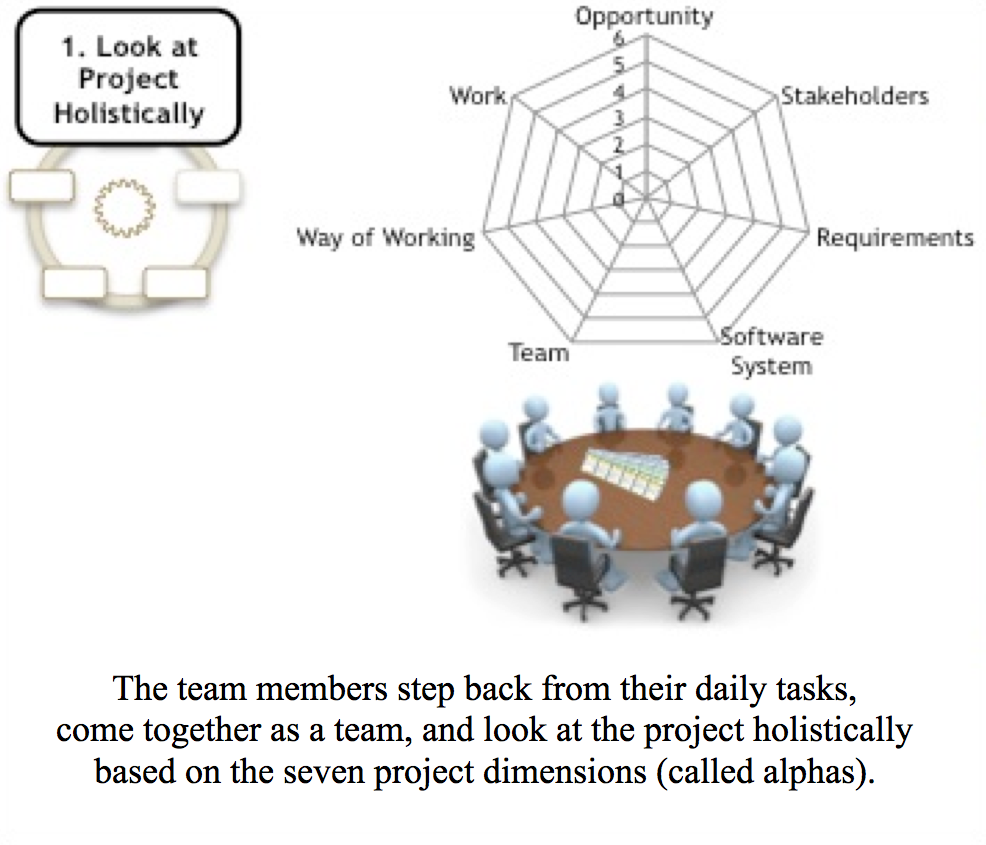
\includegraphics[width=3.2in]{reflection_meeting_images/EssenceMeetingStep1.png} & 
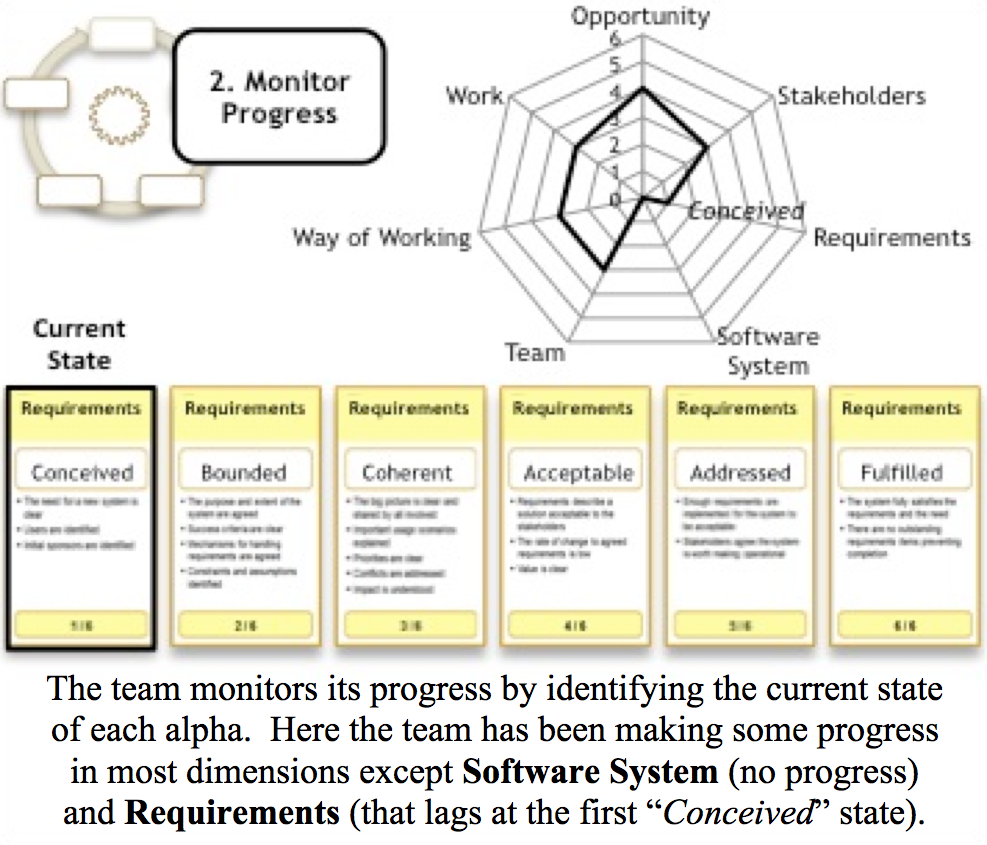
\includegraphics[width=3.2in]{reflection_meeting_images/EssenceMeetingStep2.png} \\
\hline
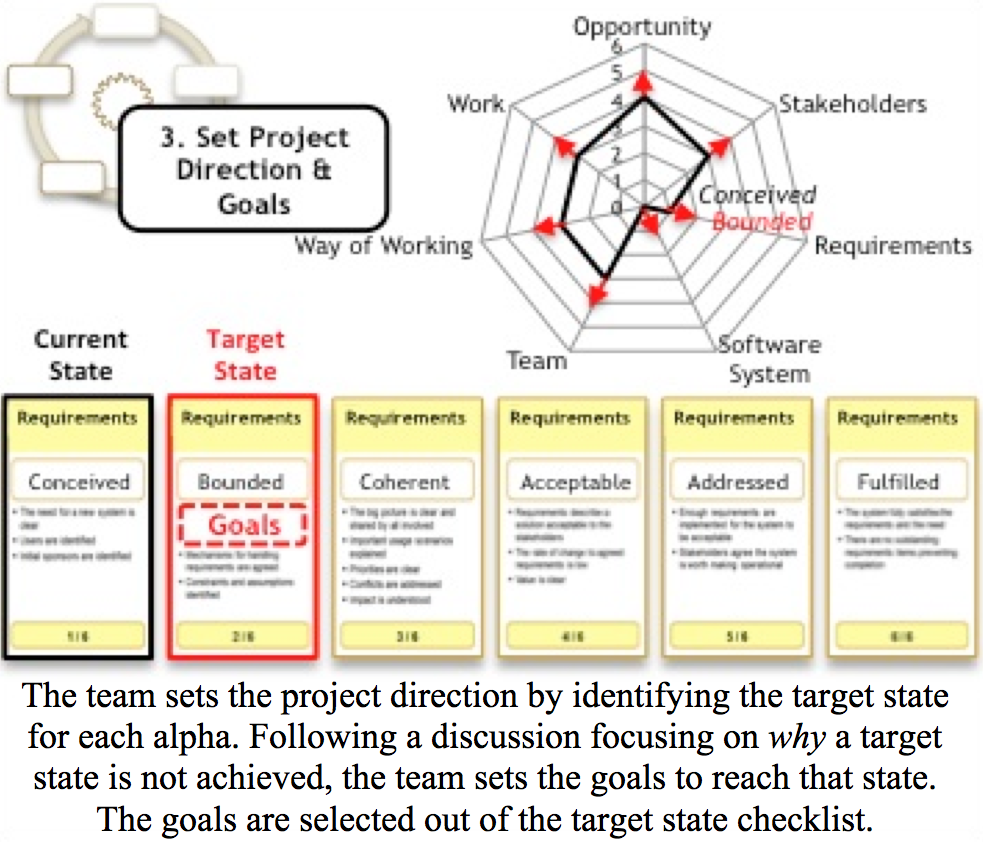
\includegraphics[width=3.2in]{reflection_meeting_images/EssenceMeetingStep3.png} &
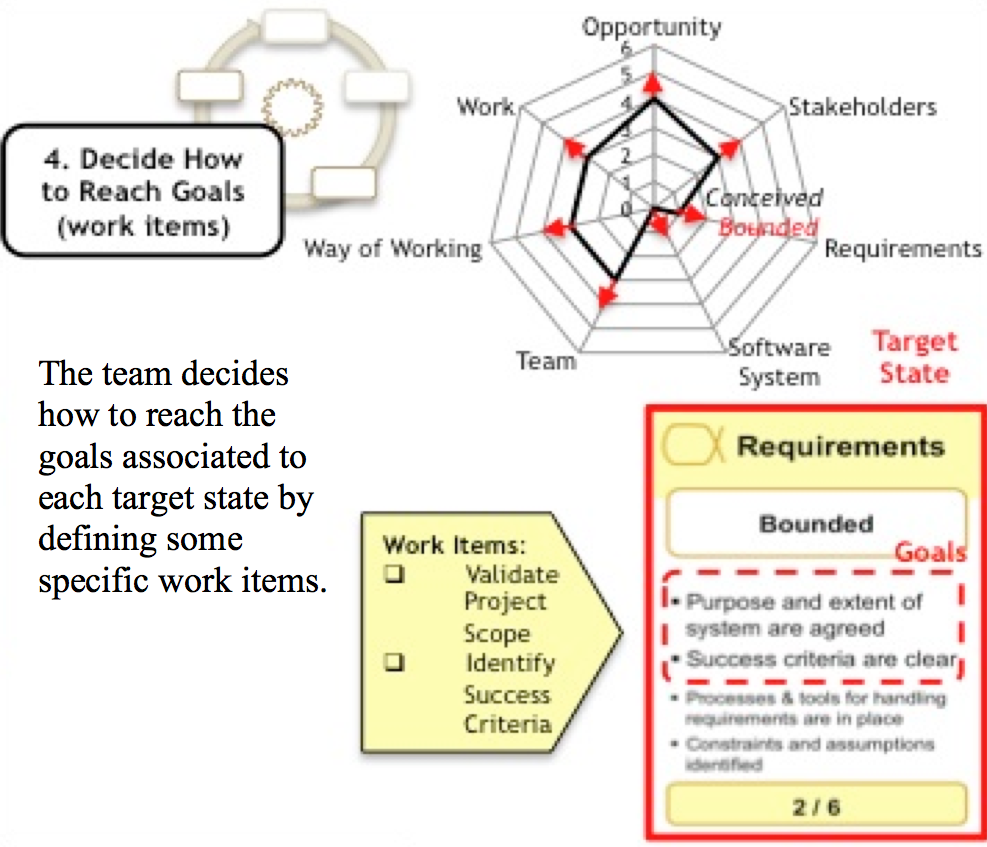
\includegraphics[width=3.2in]{reflection_meeting_images/EssenceMeetingStep4.png} \\
\hline
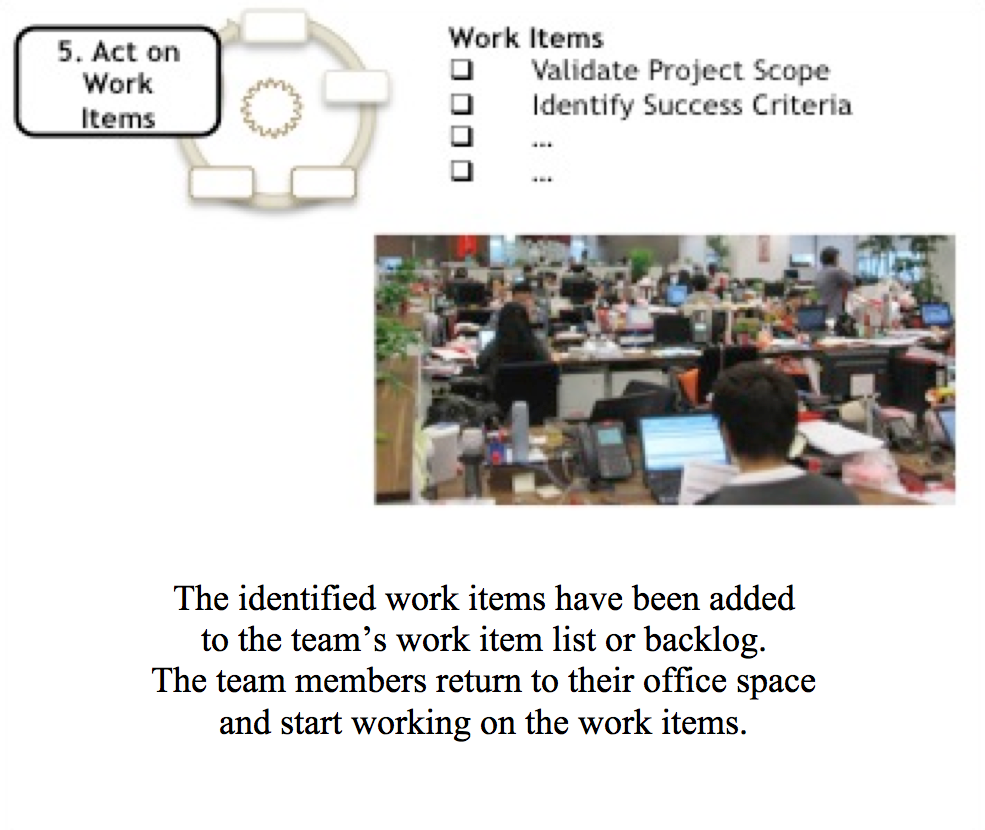
\includegraphics[width=3.2in]{reflection_meeting_images/EssenceMeetingStep5.png} &
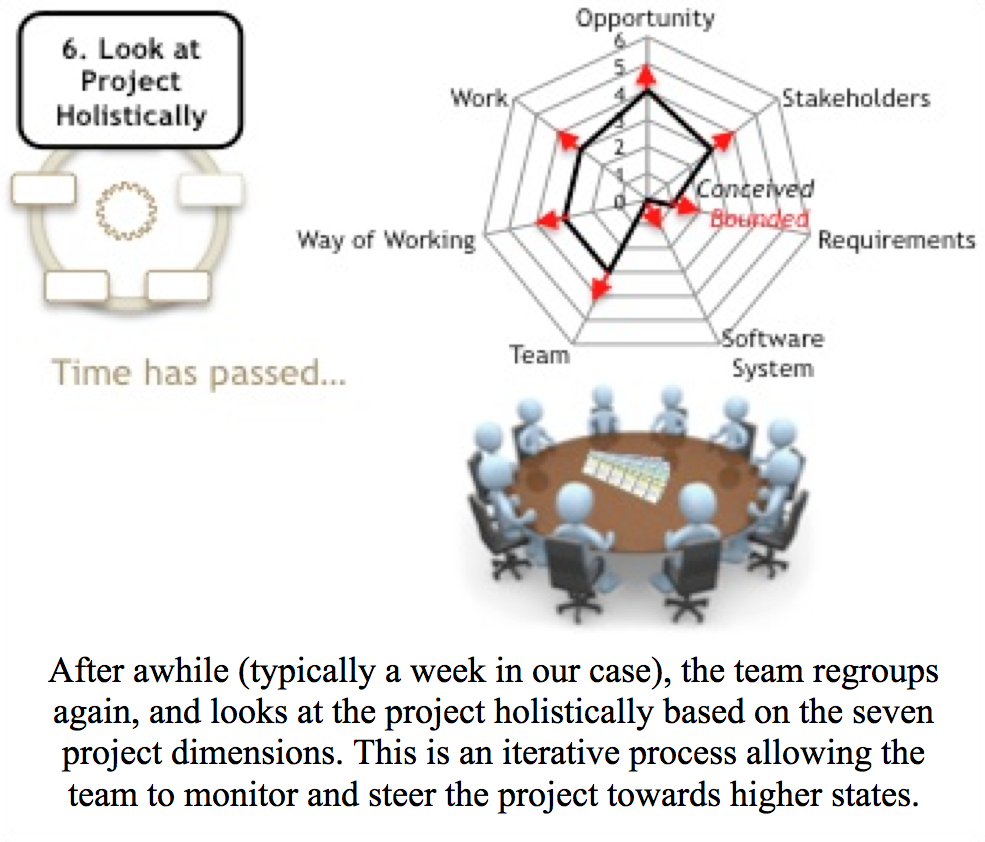
\includegraphics[width=3.2in]{reflection_meeting_images/EssenceMeetingStep6.png} \\
\end{tabular}
\label{EssenceReflectionMeetings}
\end{table*}